\section{基本不等式}
\begin{theorem}[基本不等式]
    $a>0,b>0$那么有：
    $$
        \frac{a+b}{2}\geq\sqrt{ab}
    $$
    当且仅当$a=b$时不等式取等号。
\end{theorem}
\begin{proof}法一
    \begin{align*}
             & (\sqrt{a}-\sqrt{b})^2\geq0 \\
        \iff & a+b-2\sqrt{ab}\geq0        \\
        \iff & \frac{a+b}{2}\geq\sqrt{ab}
    \end{align*}
    当且仅当$\sqrt{a}=\sqrt{b}$也即$a=b$时取等号。
\end{proof}
\begin{proof}法二
    \begin{figure}[H]
        \centering
        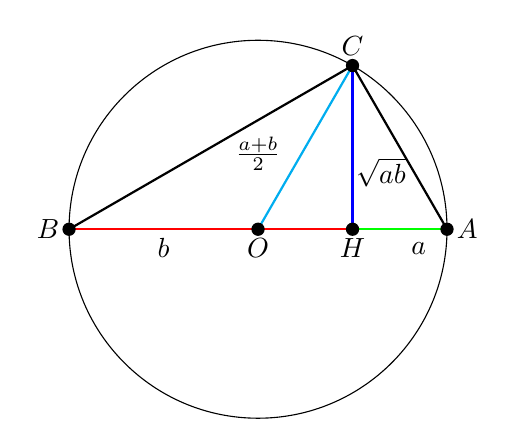
\begin{tikzpicture}[scale=1.2]
            \draw (0,0) circle (2);
            \draw[thick,color=cyan] (0,0) -- (1,{sqrt(3)});
            \draw[thick,color=red] (-2,0) -- (1,0);
            \draw[thick,color=green] (1,0) -- (2,0);
            \draw[thick] (-2,0) -- (1,{sqrt(3)});
            \draw[thick] (2,0) -- (1,{sqrt(3)});
            \draw[thick,color=blue] (1,0) -- (1,{sqrt(3)});
            \node at (-1,-0.2) {$b$};
            \node at (1.7,-0.2) {$a$};
            \node at (1.3,0.6) {$\sqrt{ab}$};
            \node at (0,0.8) {$\frac{a+b}{2}$};
            \fill (0,0) circle (2pt) node[below] {$O$};
            \fill (2,0) circle (2pt) node[right] {$A$};
            \fill (-2,0) circle (2pt) node[left] {$B$};
            \fill (1,{sqrt(3)}) circle (2pt) node[above] {$C$};
            \fill (1,0) circle (2pt) node[below] {$H$};
        \end{tikzpicture}
        \caption{基本不等式图解}
    \end{figure}
    如图所示，在$\triangle ABC$的外接圆$\odot O$中，作$CH\perp AB$。如果设$BH=b,AH=a$，那么显然有外接圆半径
    $$OC=\frac{a+b}{2}$$
    并且由相似三角形$\triangle BCH \sim \triangle CAH$可得：
    $$\frac{BH}{CH}=\frac{CH}{AH}$$
    于是
    $$CH=\sqrt{BH\times AH}=\sqrt{ab}$$
    在$\triangle OCH$内，斜边大于直角边：$OC>CH$，也即基本不等式：
    $$
        \frac{a+b}{2}\geq \sqrt{ab}
    $$
    当且仅当$H$和$O$重合的时候$a=b$，有$$\frac{a+b}{2}=\sqrt{ab}$$
\end{proof}